\subsection*{Redigering}
Redigering inddeles i en grænseflade og en tilhørende controller, som det fremgår af \autoref{fig:Redigering}. 

\begin{figure} [H]
\centering
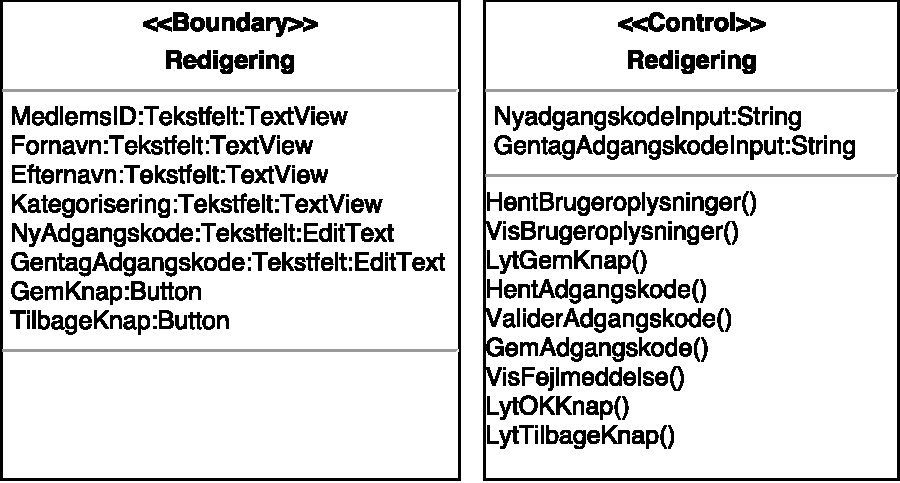
\includegraphics[width=0.9\textwidth]{figures/MVC/Redigering}
\caption{Designklasser for Redigering.}
\label{fig:Redigering}
\end{figure}


\noindent
I \textit{RedigeringGrænseflade} opstilles tekstfelter for medlemsID, fornavn, efternavn og kategorisering. Derudover opstilles tekstfelter for ny adgangskode og gentag adgangskode, hvor brugeren kan redigere adgangskoden. Dertil er der en gem knap og en tilbage knap, af typen button. Gem knappen indikere ved tryk at brugeren ønsker at gemme den nye adgangskode. 


Til \textit{RedigeringGrænsefladen} er der opstillet en \textit{RedigeringController}, som har til formål at vise informationer om brugeren. Derudover lytter den på gem knappen, hvis denne trykkes, sammenligner controlleren de indtastede adgangskoder. Er disse ens sender controlleren den  nye adgangskode til databasen. Controlleren lytter på om tilbage knappen trykkes på, hvis dette sker vises den forrige grænseflade.  

